%!TEX root = /Users/kevin/SkyDrive/KTH Work/LaTeX Reports/Atomic Nucleus Revised/Atomic Nucleus.tex
\section{Theory} 

% (fold)
\label{sec:theory} In both of these radioactive isotopes, beta and gamma decay are present. The beta decay in Cesium and Strontium are both $\beta^-$ decay, as opposed to $\beta^+$, and is given by 

\begin{equation}
	^{A}_{Z}P \to _{Z-1}^{~~~A}D + \beta^- + \bar{\nu}_e \nonumber 
\end{equation}%(beta decay equation)

where $P$ and $D$ represent the parent and daughter atoms and $ \bar{\nu}_e$ is an anti-neutrino. The anti-neutrino is important because it shares the total energy with the beta particle. This leads to a continuous distribution of energies instead of discrete values, see Figure~\ref{fig:Figures_betabi210}.

\begin{figure}
	[bp] \centering 
	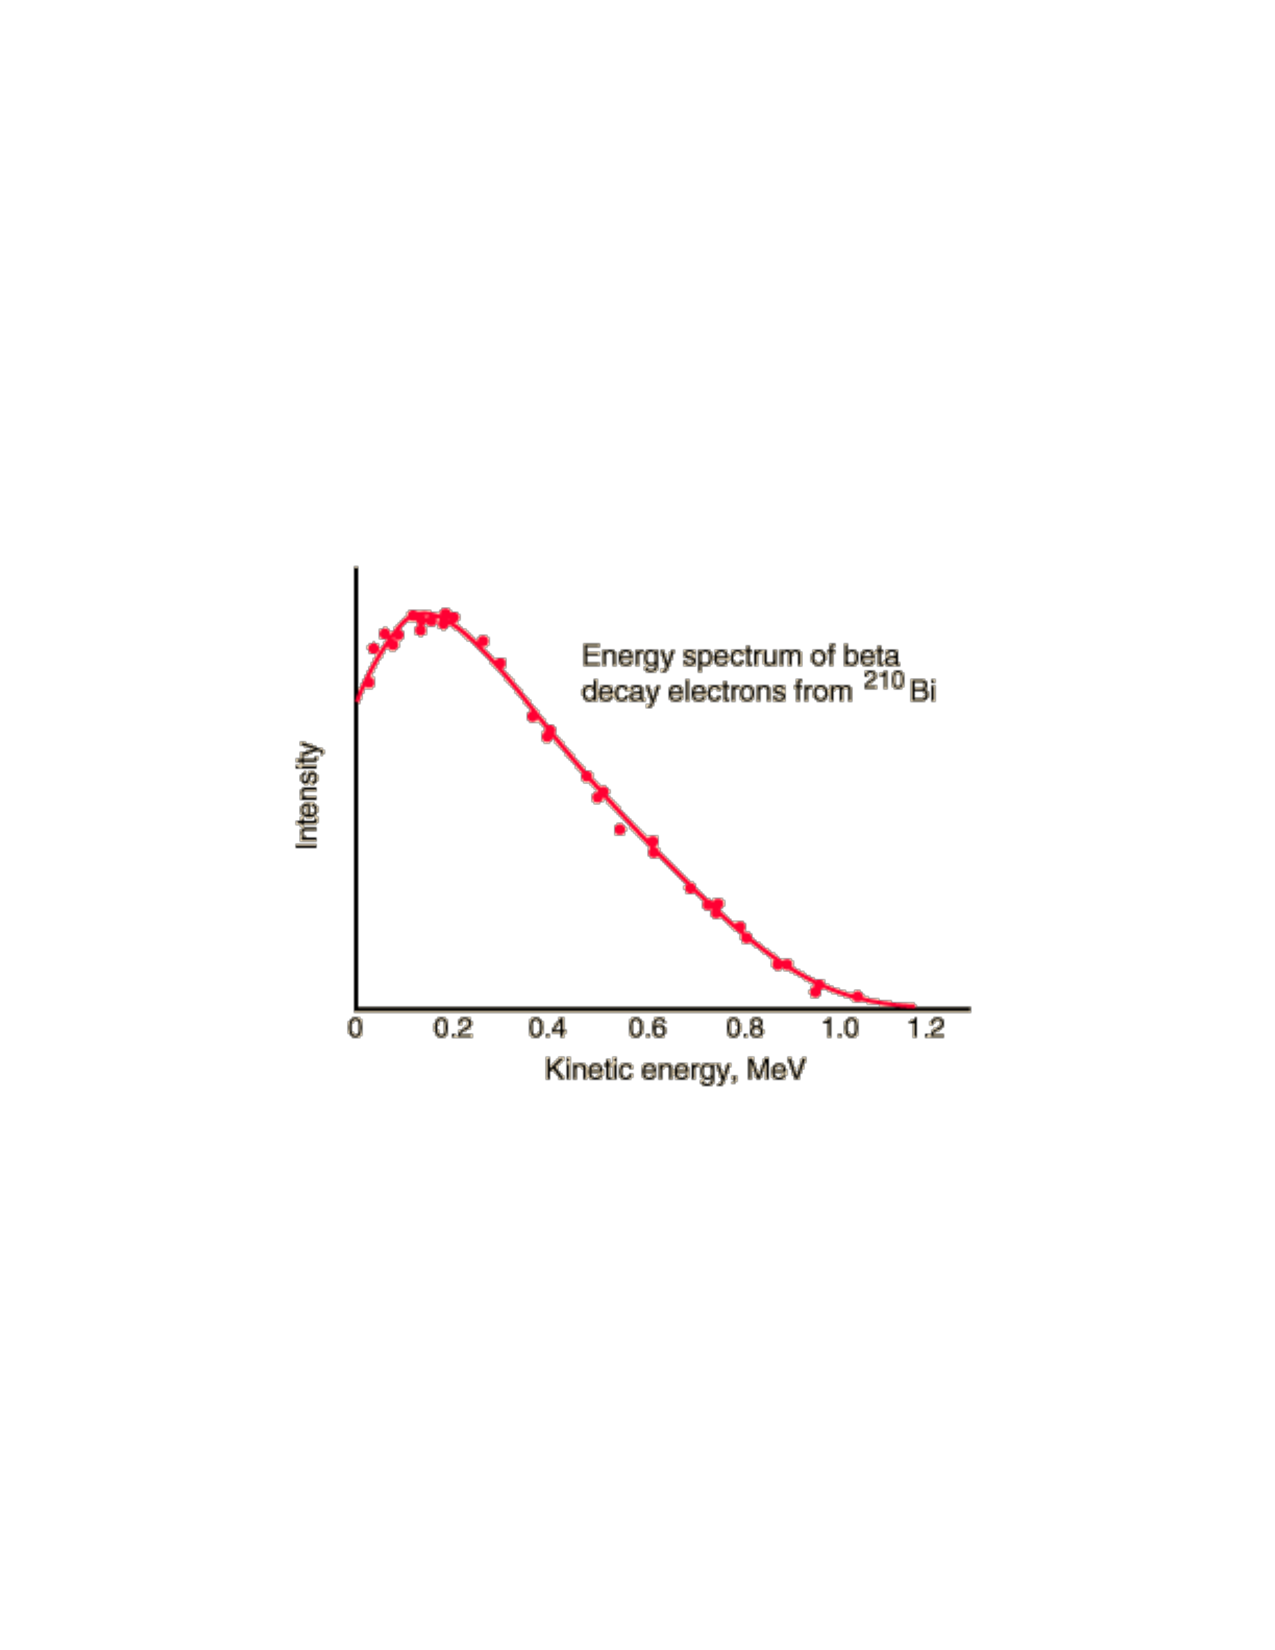
\includegraphics[width=.5
	\textwidth]{./Figures/betabi210.pdf} \caption{General beta decay energy distribution\cite{Neary28031940}} \label{fig:Figures_betabi210} 
\end{figure}%(General Beta Energy Distribution)

Figure~\ref{fig:Figures_137CsDecayScheme} shows the beta decay of cesium with probabilities of each process.
\begin{figure}
	[tbp] \centering 
	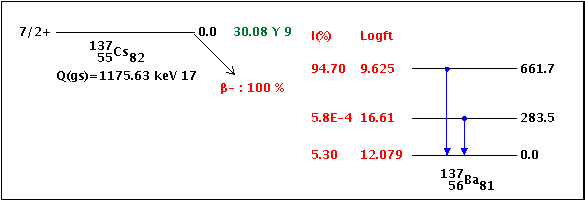
\includegraphics[width=.9
	\textwidth]{./Figures/137CsDecayScheme.png} \caption{Decay Scheme of $^{137}\textrm{Cs}$.\cite{nndc}} \label{fig:Figures_137CsDecayScheme} 
\end{figure}%(fig:Figures_137CsDecayScheme)
Each of these energies must be seen as the maximum energy a beta particle can have because it shares the total energy with an anti-neutrino. From these energies and associated probabilities, we can expect an energy distribution containing one gaussian distribution and two beta distributions with different maximum energy values. Internal conversion occurs $10\%$ of the time at an excited state of Barium, $E=661.7~$keV in Figure~\ref{fig:Figures_137CsDecayScheme}. The other $90\%$ of the time, gamma rays will be emitted. Internal conversion means that an orbiting electron receives the excess energy from a transition between states in the same nucleus $E=661.7~\text{keV}-E_b$, where $E_b=37.441~\text{keV}$ is the binding energy of the electron. It is emitted with an exact amount of energy every time, $E=624.3~\text{keV}$.  However, the collected data will be a normally distributed because of the errors in the measurement equipment and the different path lengths for each electron due to scattering.  

In Figures~\ref{fig:Figures_137CsDecayScheme}, \ref{fig:Figures_90SrDecay}, and \ref{fig:Figures_90YDecay}, I(\%) is the radiation intensity and indicates the probability of occurence.  Logft is given by, $\log(f(Z,E_0)t_{1/2})$, where $f(Z,E_0)$ is the fermi integral, $E_0$ is the end point energy, and $t_{1/2}$ is the half-life.  This value classifies $\beta$ transitions and depends on the probability of decay, half-life, and energy.\cite{nndc} 

A similar beta decay process occurs for Strontium, except it decays through two elements before becoming stable. Both of these decay processes emit beta particles, but does not have internal conversion. First, Strontium decays to Yttrium, $^{90}\text{Y}$, another radioactive isotope (see Figure~\ref{fig:Figures_90SrDecay}). Yttrium then decays to a stable isotope of Zirconium, $^{90}\text{Zr}$ (see Figure~\ref{fig:Figures_90YDecay}).

\begin{figure}
	[tbp] \centering 
	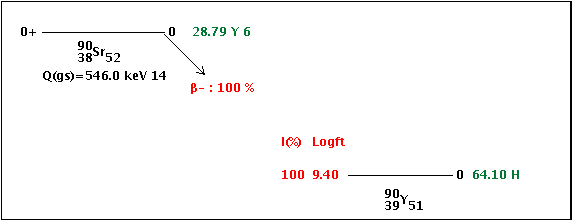
\includegraphics[width=.9
	\textwidth]{Figures/90SrDecay.png} \caption{Decay Scheme of Strontium} \label{fig:Figures_90SrDecay} 
\end{figure}%(fig:Figures_90SrDecay)
\begin{figure}
	[tbp] \centering 
	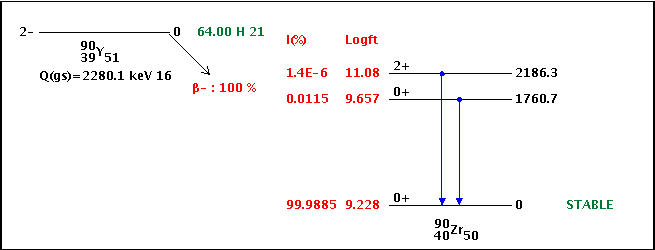
\includegraphics[width=.9
	\textwidth]{Figures/90YDecay.png} \caption{Decay Scheme of Yttrium.  Two of the three decay processes shown have extremely low probabilities ($\ll 1\%$) and therefore, the only process considered has an energy, $\text{E}=2280.1~\text{keV}$.} \label{fig:Figures_90YDecay} 
\end{figure}%(fig:Figures_90YDecay)

% Repeat for decay processes of Strontium except it has two decay processes that occur. Cesium produces a discrete energy value at \textbf{value} This property of Cesium is used in the experimental setup for calibration. 

From this energy distribution, we can determine the beta particles ability to penetrate materials and in this experiment we will use aluminium and plastic. We adjust the thickness of the material and the material to determine a thickness needed to stop beta particles of a certain energy. Every time we add thickness to the materials, we expect the energy distributions to shift towards lower energies.  Electrons 
% In this experiment, we will also make the assumption that the electrons take a direct path from the radioactive material to the detector. 


% section theory (end)